\documentclass[article, 11pt]{article}
\usepackage{comment} % enables the use of multi-line comments (\ifx \fi) 
\usepackage{epsfig}
\graphicspath{ {./photos/} }
\usepackage{lipsum} %This package just generates Lorem Ipsum filler text. 
\usepackage{fullpage} % changes the margin
\usepackage{graphicx}
\usepackage{siunitx}
\usepackage{listings}
\usepackage{amsmath}
\usepackage{multicol,caption}
\usepackage{wrapfig}
\usepackage[T1]{fontenc}
\usepackage{setspace} 
\usepackage{float}
\usepackage{subcaption}



\usepackage{dcolumn}% Align table columns on decimal point
\usepackage{bm}% bold math
\usepackage{amssymb}
\usepackage{epsf}
\usepackage{subfigure}
%\usepackage{flafter}
\usepackage{float}
\usepackage{epstopdf}
\usepackage{color}
\usepackage{subeqnarray}
\usepackage{mathrsfs}
\usepackage[colorlinks=true, pdfstartview=FitV, linkcolor=black, citecolor=blue, urlcolor=blue]{hyperref}





\newcommand{\be}{\begin{equation}}
\newcommand{\ee}{\end{equation}}
\newcommand{\ben}{\begin{eqnarray}}
\newcommand{\een}{\end{eqnarray}}


% \graphicspath{ {./images/} }
\newenvironment{Figure}
 {\par\medskip\noindent\minipage{\linewidth}}
 {\endminipage\par\medskip}
%\setmarginsrb{1 cm}{0.7 cm}{1 cm}{1.5 cm}{1 cm}{0.5 cm}{0.5 cm}{1 cm}

\title{
    \begin{spacing}{0.1}
        \rule{\textwidth}{0.5pt}
        \rule{\textwidth}{0.5pt}
    \end{spacing}
    \vspace{1cm}
    \Huge\textbf{CS 301 \\High-Performance Computing}
    \vspace{0.7cm}
    \begin{spacing}{0.1}
        \rule{\textwidth}{0.5pt}
        \rule{\textwidth}{0.5pt}
    \end{spacing}

    \vspace{6cm}
    {\Huge{\underline{Lab 3: Problem A1}}}
}

\author{
    \vspace{5cm}
    \\Kunal Hotwani (202001468)
    \\Harsh Patel (202001173)
}


\begin{document}
\maketitle

\newpage
\tableofcontents

%%%%%%%%%%%%%%%%%%%%%%
\newpage
\section{Introduction}



\subsection{Brief description of the problem.}


\textbf{ Problem A-1 ->} → Conventional matrix multiplication.

\vspace{3mm}

 Conventional Matrix Multiplication is a matrix multiplication method with time complexity $O(n^3)$. In this question, we have taken all the six possible combinations of arranging the three loops to obtain six different outputs and compared them with each other.

\vspace{1mm}


 Our objective is to compare the algorithms to obtain the best method which gives maximize the utilization of the processor.

 

\subsection{The complexity of the algorithm (serial).}

\vspace{3mm} 
The time complexity of the code is $O(n^3)$ and the space complexity is $O(n^2)$.

\vspace{1mm}
In the code, the for loop is the main source of computation and the three for lops run n times, where n is the number of terms in the matrix. Hence, the time complexity is $O(n^3)$.

\vspace{1mm}
No extra variables other than the matrix are being used, making the space complexity $O(n^2)$


\section{Hardware Details}

\subsection{Hardware Details of LAB207 Computer}

\begin{itemize}
    \item CPU - 4
    \item Socket - 1
    \item Cores per Socket - 4
    \item Size of L1 cache - 64KB
    \item Size of L2 cache - 256KB
    \item Size of L3 cache - 6MB
\end{itemize}

\subsection{Hardware Details of Cluster}

\begin{itemize}
    \item CPU - 16
    \item Socket - 2
    \item Cores per Socket - 8
    \item Size of L1 cache - 64KB
    \item Size of L2 cache - 256KB
    \item Size of L3 cache - 20MB
\end{itemize}


%%%%%%%%%%%%%%%%%%%%%%

\section{PART 1: LAB207 Computer}

\subsection{Profiling information}
\begin{figure}[H]
\centering
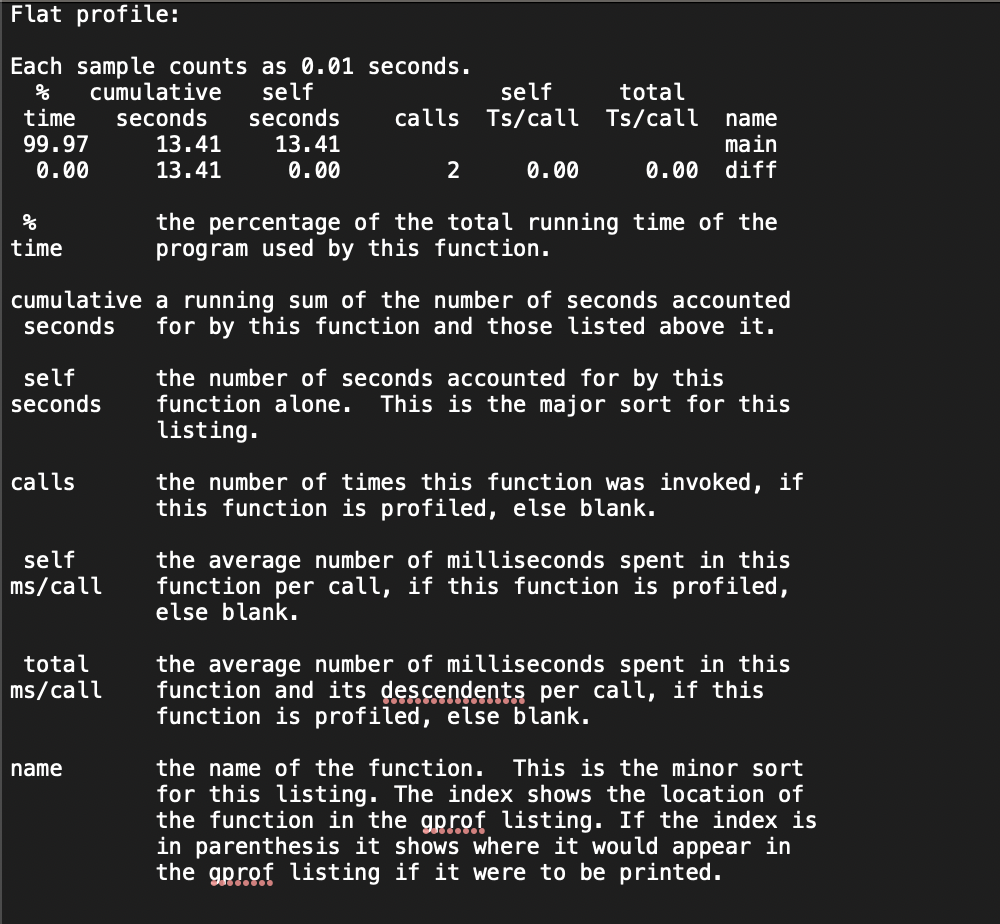
\includegraphics[width = 3 in]{1_PC.png}~
\caption{Profiling information - PC} \label{Q1_profile_PC.png}
\end{figure}

\subsection{Graphical Results}

\begin{figure}[h]
  \centering
  \begin{subfigure}[b]{0.45\textwidth}
    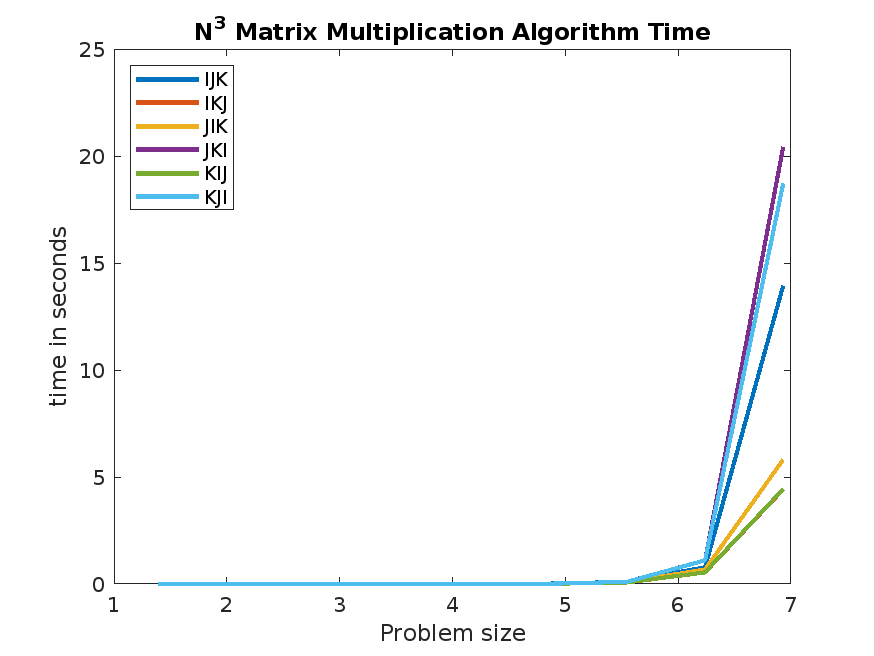
\includegraphics[width=\textwidth]{Q1_Algo_PC.png}
    \caption{Algorithm Time.}
    \label{fig:image1}
  \end{subfigure}
  \begin{subfigure}[b]{0.45\textwidth}
    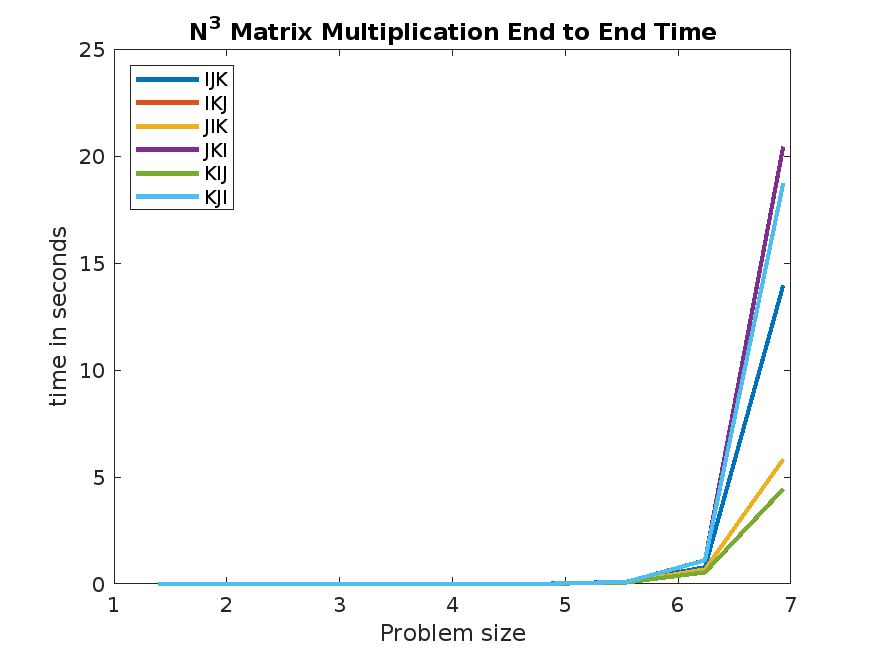
\includegraphics[width=\textwidth]{Q1_EndtoEnd_PC.png}
    \caption{End to End Time}
    \label{fig:image2}
  \end{subfigure}
  \caption{Results for Lab207 PC}
  \label{fig:entire_figure}
\end{figure}


\section{PART 2: Cluster}

\subsection{Profiling information}
\begin{figure}[H]
\centering
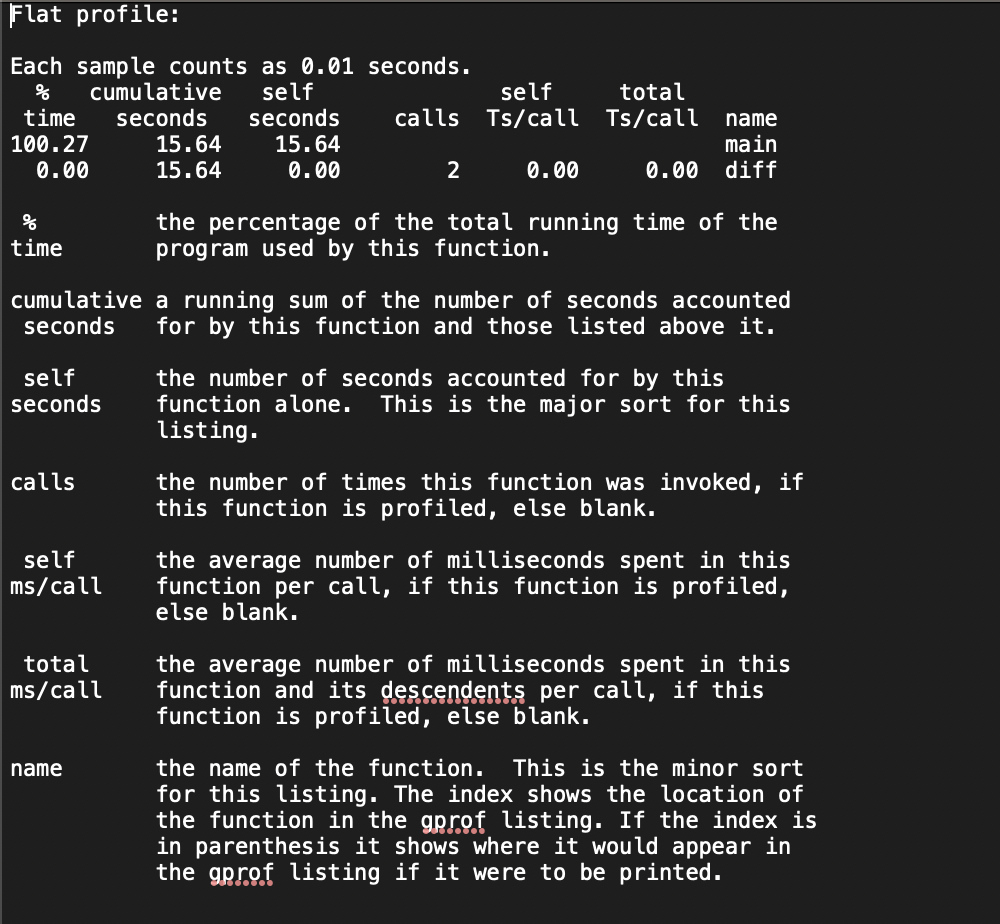
\includegraphics[width = 3 in]{1_CLUSTER.png}~
\caption{Profiling information - Cluster} \label{Q1_Profile_Cluster.png}
\end{figure}

\subsection{Graphical Results}
\begin{figure}[h]
  \centering
  \begin{subfigure}[b]{0.45\textwidth}
    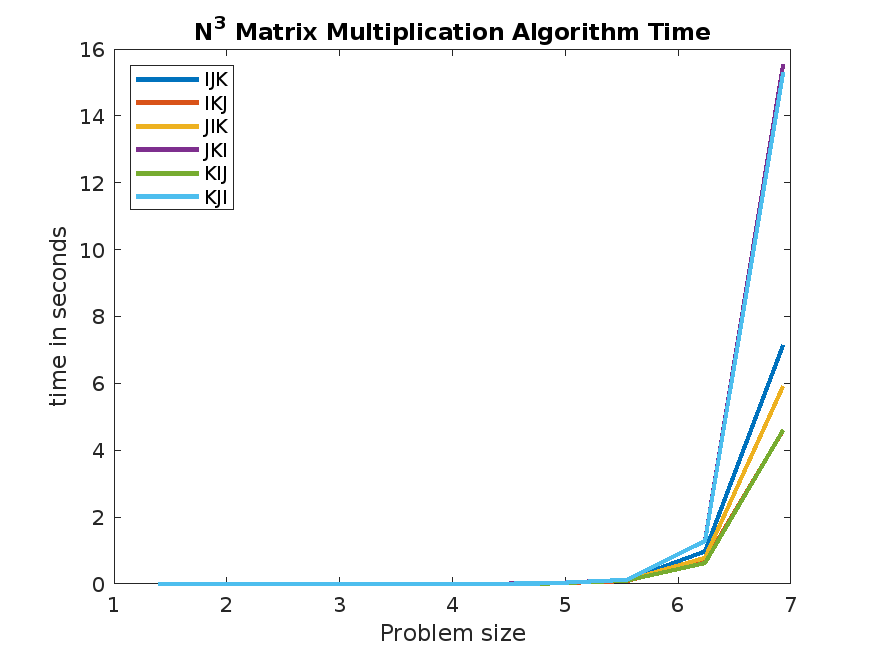
\includegraphics[width=\textwidth]{Q1_Algo_CLUSTER.png}
    \caption{Algorithm Time.}
    \label{fig:image1}
  \end{subfigure}
  \begin{subfigure}[b]{0.45\textwidth}
    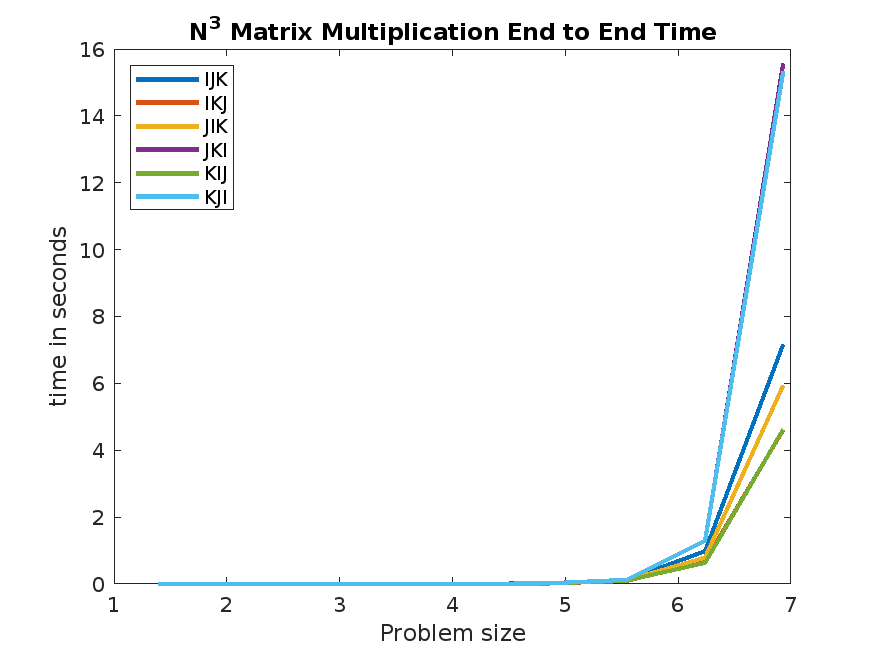
\includegraphics[width=\textwidth]{Q1_EndtoEnd_CLUSTER.png}
    \caption{End to End Time}
    \label{fig:image2}
  \end{subfigure}
  \caption{Results for HPC Cluster}
  \label{fig:entire_figure}
\end{figure}


\end{document}